\section{NN+X}
\subsection{改进思路}
计算机视觉中的目标检测问题是训练模型,给予该模型一张图片,模型将图片内特定物体框出,其效果如~\ref{fig:rcnn1}
\begin{figure}[htb]
\centering
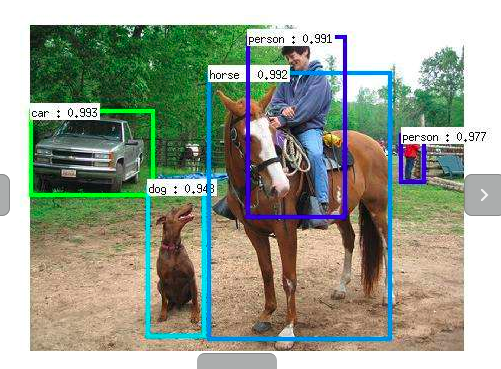
\includegraphics[scale=0.4]{../figures/rcnn1.png} 
\caption{RCNN 效果}
\label{fig:rcnn1}
\end{figure}
训练模型所使用的数据中,输入数据为原始图片,输出为标签区域坐标(label region)以及该边框所框的物体类别(label)。在该领域上,常采用RCNN(Region Convolutional Neural Network)去建立模型。RCNN算法流程图如~\ref{fig:rcnn2}。RCNN通过图像处理方法生成多个候选框(Candidate region),并对候选框做缩放,得到同样尺寸的图像,之后放入特征提取层中提取特征,再拉长为列向量。此时,RCNN需要两轮训练,一轮是针对softmax层的(如图中PATH 1),该层用于微调候选框;另一层是针对SVM的(如图中PATH 2),用于该框所属类别的分类。由于SVM是二分类器,因而还使用了OvR策略,构建和类别数一样多的分类器个数。训练softmax层和训练SVM的标签是有些许不同,这是由RCNN所要解决的问题决定的,在此处并不进行讨论。在RCNN中,由于直接采用softmax会比采用SVM精度低,而且SVM适用于少样本的训练,所以采用SVM替代了softmax。
\begin{figure}[htb]
\centering
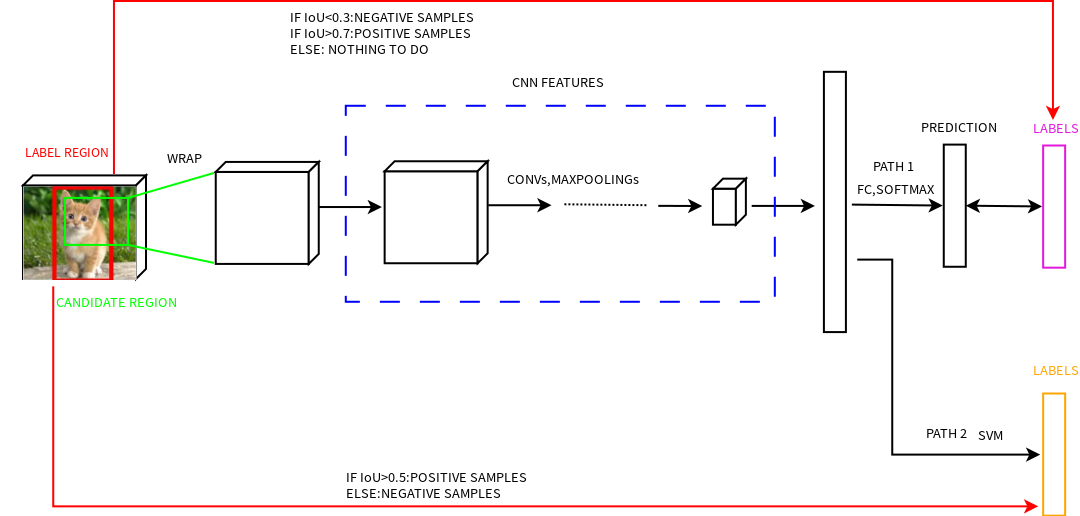
\includegraphics[scale=0.4]{../figures/rcnn_2.png} 
\caption{RCNN算法流程}
\label{fig:rcnn2}
\end{figure}

从RCNN带来的想法是神经网络与传统机器学习模型的融合。由于本问题是一个分类问题,卷积神经网络强大之处在于提取并学习图像特征,从而得到远低于图像维度的特征向量,而SVM在小样本的分类问题中有很好的性能。若是采用卷及神经网络提取特征得到特征向量后,采用SVM分类器分类可能能够提升模型的性能,本文的想法是神经网络带softmax进行训练,在调整完网络之后,采用某种分类算法(记为算法X)去替换softmax层,并训练算法X,算法流程如图~\ref{fig:x1}。
为了探究此种替换是否有提升,论文也将探讨多种神经网络:BP神经网络(选取表~\ref{fig:bpx1}的BP神经网络结构)、VGGNet所更改的网络(选取表~\ref{fig:cnn7}的CNN-A到CNN-D的结构)、Inception结构(选取图~\ref{fig:inception2}和~\ref{fig:inception3}的CNN-E和CNN-F的结构),与分类器算法X:SVM,决策树,随机森林的组合。

\begin{figure}[htb]
\centering
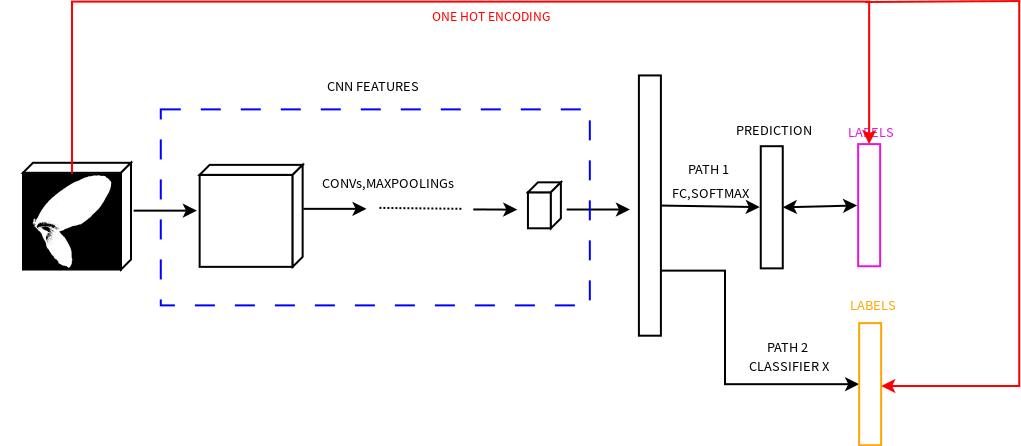
\includegraphics[scale=0.4]{../figures/rcnn_4.png} 
\caption{CNN+X模型}
\label{fig:rcnn2}
\end{figure}

\begin{table}[htb]
\centering
\caption{BP-A,BP-B,BP-C,BP-D模型概况}
\begin{tabular}{ccccc}
\toprule[2pt]
model & BP-A & BP-B & BP-C & BP-D \\ 
\midrule[1pt]
隐含层 & 1000 & 1000 & 500 & 500 \\ 
所用数据集 & I64 & I96 & I96 & I96 \\ 
学习率 & 0.03 & 0.03 & 0.03 & 0.03 \\ 
优化函数 & MGD & MGD & MGD & MGD \\ 
正则化参数 & 0 & 0 & 0 & 0.0001 \\ 
\midrule[1pt]
准确率 & 0.518188 & 0.522655 & 0.516273 & 0.49649 \\ 
\bottomrule[2pt]
\end{tabular} 
\label{table:bpx2}
\end{table}

\subsection{BP神经网络+X}
为了对比改进后模型的性能,首先要排除SVM在I64,I96,I128就有异常好的性能的可能性(比如超越卷积神经网络的准确率)。先在I64,I96,I128上进行SVM的分类,其结果如图~\ref{table:bpx1}
\begin{table}[htb]
\centering
\caption{SVM在I64,I96,I128上的分类结果准确率。其中,svm-k,k代表核函数类型}
\begin{tabular}{ccccc}
\toprule[2pt]
数据集 & svm-linear & svm-poly & svm-rbf & svm-sigmoid \\ 
I64 & 0.361199 & 0.524569 & 0.486280 & 0.081685 \\ 
I96 & 0.388641 & 0.534142 & 0.507339 & 0.086790 \\ 
I128 & 0.373325 & 0.559668 & 0.507977 & 0.356733 \\ 
\bottomrule[2pt]
\end{tabular}
\label{table:bpx1}
\end{table} 
其中,多项式核svm能够达到较高的准确率。

	
接下来,在BP-A到BP-D中,将softmax换成SVM,有表~\ref{table:bpx3}
\begin{table}[htb]
\centering
\caption{第一列为原始的BP-A,BP-B,BP-C,BP-D准确率,第二列为svm在I64,I96上的准确率,第三到第六列为BP-A,BP-B,BP-C,BP-D中将softmax层换成SVM,并依次选取linear,poly,rbf,sigmoid核后的准确率}
\begin{tabular}{ccccccc}
\toprule[2pt]
\ &softmax &svm-poly &bpsvm-linear & bpsvm-poly & bpsvm-rbf & bpsvm-sigmoid \\ 
BP-A & 0.518188 & 0.524569 & 0.538609 & 0.576260 & 0.587109 & 0.081685 \\ 
BP-B & 0.522655 & 0.534142 & 0.530951 & 0.577537 & 0.590938 & 0.075303 \\ 
BP-C & 0.516273 & 0.534142 & 0.507339 & 0.541799 & 0.580728 & 0.066369 \\ 
BP-D & 0.49649 & 0.534142 & 0.529675 & 0.572431 & 0.594129 & 0.356733 \\ 
\bottomrule[2pt]
\end{tabular} 
\label{table:bpx3}
\end{table}

为了更为直观展现结果,表~\ref{table:bpx3}对应的图~\ref{fig:bpx1}如下
\begin{figure}[htb]
\centering
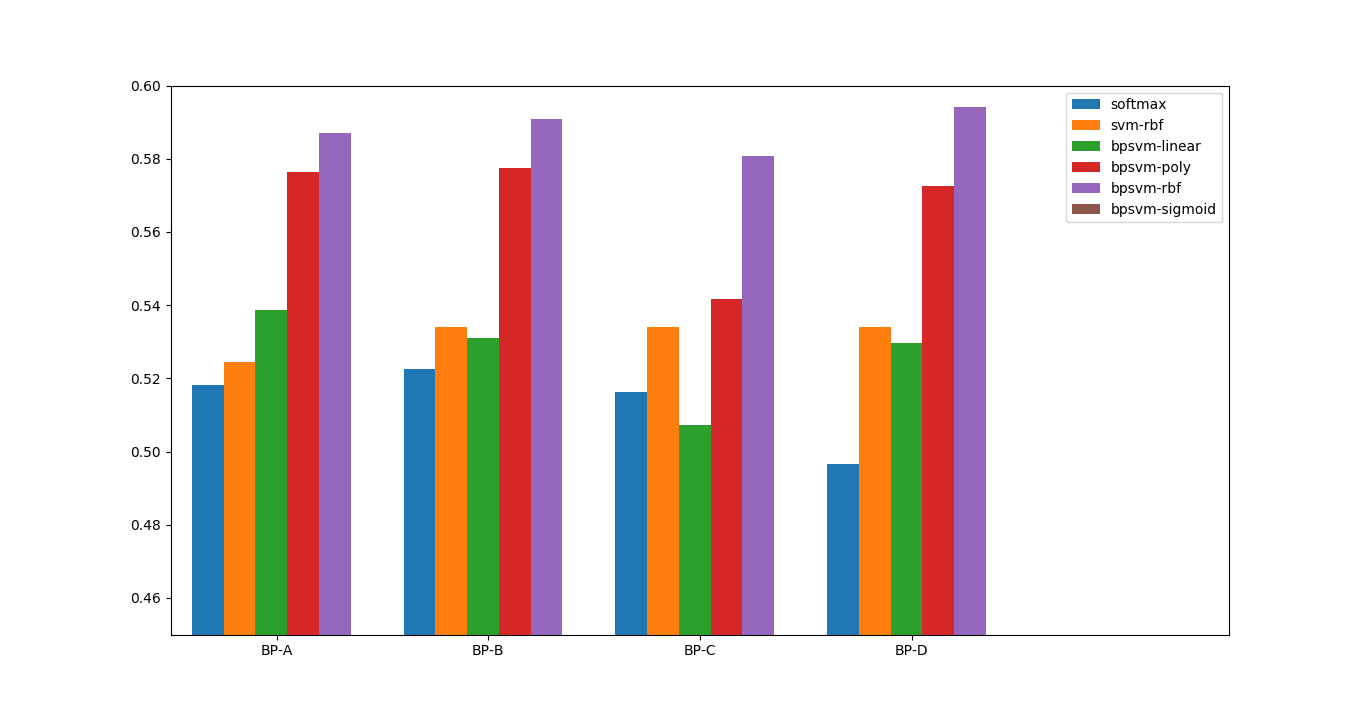
\includegraphics[scale=0.5]{../figures/NN_svm1.png} 
\caption{原始的BP-A,BP-B,BP-C,BP-D,SVM,与用SVM替换BP-A,BP-B,BP-C,BP-D中softmax层所得的准确率图}
\label{fig:bpx1}
\end{figure}

可以看出,当采用高斯核函数的SVM替换BP神经网络的softmax层,能够显著提高模型效果。相比与原来带有softmax层的BP神经网络,其准确率提高了6.4\%到9.7\%左右,相比于原来带多项式核函数的SVM,其准确率提高了4.7\%到6.3\%左右。从结果上看,似乎BP神经网络与SVM的结合有成效,下面将用CART树和随机森林来进一步探究BP神经网络+X的有效性。下面使用CART树代替softmax,有结果如表~\ref{table:bpx4},为了更为直观展现结果,表~\ref{table:bpx4}对应的条形图~\ref{fig:bpx2}如下
\begin{table}[htb]
\centering
\caption{第1列为原始的BP-A,BP-B,BP-C,BP-D准确率,第2列为bpsvm-rbf准确率,第3到6列为用CART树代替softmax的准确率,其中mdh代表最大深度。}
\begin{tabular}{cccccccc}
\toprule[2pt]
model  & softmax & bpsvm-rbf & bpCART-mdh:5 & bpCART-mdh:10 & bpCART-mdh:15 & bpCART-mdh:20\\ 
BP-A & 0.518188 & 0.587109 & 0.414167 & 0.417358 & 0.408424 & 0.411615\\ 
BP-B & 0.522655 & 0.590938 & 0.416720 & 0.398851 & 0.387364 & 0.391078\\ 
BP-C & 0.516273 & 0.580728 & 0.353542 & 0.337588 & 0.325463 & 0.327378\\ 
BP-D & 0.49649 & 0.594129 & 0.395662 & 0.398851 & 0.389917 & 0.391193\\ 
\bottomrule[2pt]
\end{tabular} 
\label{table:bpx4}
\end{table}

\begin{figure}[htb]
\centering
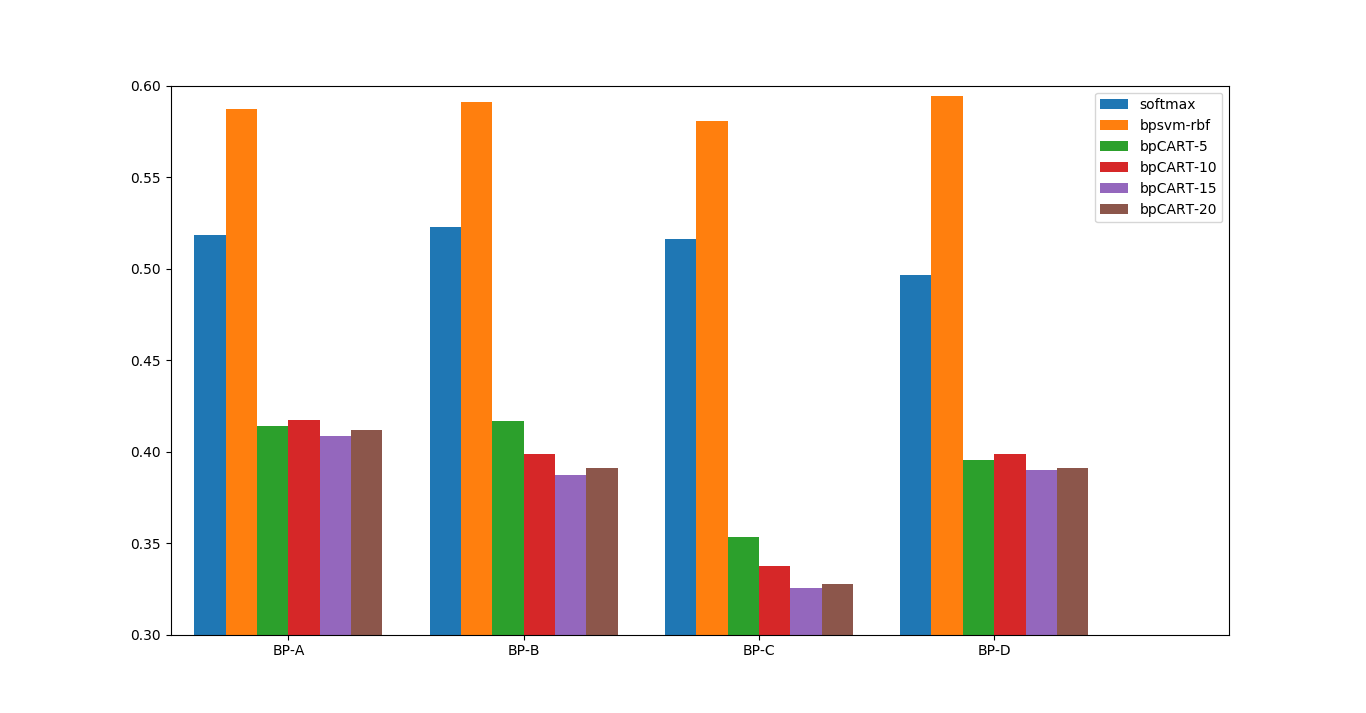
\includegraphics[scale=0.5]{../figures/NN_tree1.png} \\
\caption{原始的BP-A,BP-B,BP-C,BP-D,bpsvm-rbf,与用不同深度的CART替换softmax层所得的准确率图}
\label{fig:bpx2}
\end{figure}

当X为CART树时,效果并不令人满意,有可能是树模型的弊端造成的,而非是BP神经网络+X的结构所带来的问题。为了克服树的弊端,选取随机森林,对树模型进行集成,可大大提高树模型的性能。下面讨论X为随机森林时,BP神经网络+X的模型性能。结果如表~\ref{table:bpx5},对应图~\ref{fig:bpx3}

\begin{table}[htb]
\centering
\caption{第1列为原始的BP-A,BP-B,BP-C,BP-D准确率,第2列为nsvm-rbf准确率,第3到6列为用随机森林代替softmax的准确率,其中,n代表随机森林包含的树桩个数。}
\begin{tabular}{cccccc}
\toprule[2pt]
model & softmax & bpsvm-rbf & bprf-n:20 & bprf-n:50 & bprf-n:80 \\ 
BP-A & 0.518188 & 0.587109 & 0.544352 & 0.552010 & 0.573070 \\ 
BP-B & 0.522655 & 0.590938 & 0.530313 & 0.559668 & 0.574346 \\ 
BP-C & 0.516273 & 0.580728 & 0.504786 & 0.534780 & 0.555839 \\  
BP-D & 0.49649 & 0.594129 & 0.523293 & 0.561583 & 0.555839 \\ 
\midrule[2pt]
model & bprf-n:110 & bprf-n:140 & bprf-n:170 & bprf-n:200 & bprf-n:230 \\ 
BP-A & 0.574346 & 0.569879 & 0.577537 & 0.580089 & 0.574984 \\ 
BP-B & 0.569879 & 0.586471 & 0.596043 & 0.583918 & 0.575622 \\ 
BP-C & 0.545629 & 0.557754 & 0.550734 & 0.562221 & 0.569241 \\ 
BP-D & 0.560944 & 0.573070 & 0.576899 & 0.580089 & 0.579451 \\ 
\bottomrule[2pt]
\end{tabular} 
\label{table:bpx5}
\end{table}

当X为随机森林时,其体现出了集成学习的优势,准确率相对于CART树,准确率高出14\%以上,并且在BP-B的170个树桩的随机森林上,准确率达到59.6\%,超越bpsvm-rbf的59.1\%的准确率,其性能比bpsvm-rbf稍低,相比与原来带有softmax层的BP神经网络,其准确率提高了4.6\%到8.4\%左右。

\begin{figure}[htb]
\centering
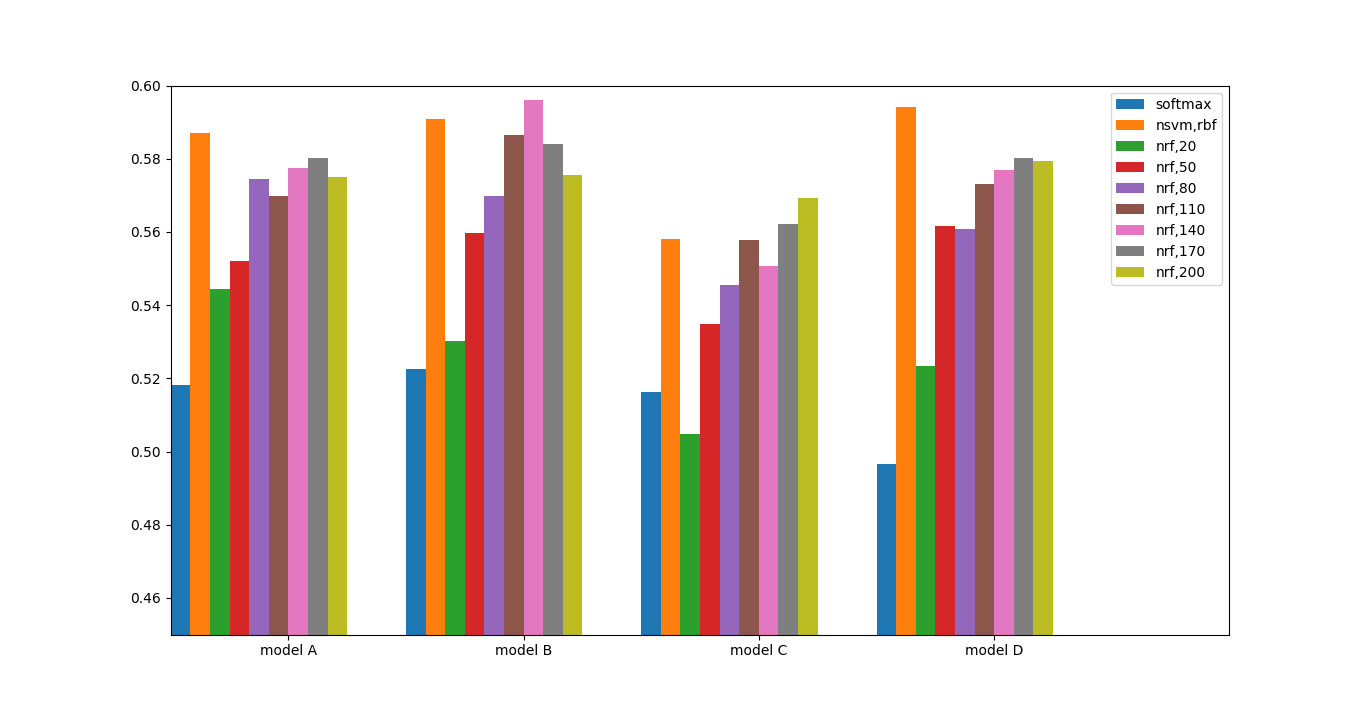
\includegraphics[scale=0.5]{../figures/NN_rf1.png} \\
\caption{原始的 BP-A,BP-B,BP-C,BP-D,bpsvm-rbf,与用包含不同树桩个数的随机森林替softmax 层所得的准确率图}
\label{fig:bpx3}
\end{figure}


\subsection{CNN+X}
对与卷及神经网络与分类器X的融合,其算法原理如图~\ref{fig:rcnn2},首先考虑svm与VGGNet所更改的网络的融合,其结果如表~\ref{table:cnnx1}
\begin{table}[htb]
\centering
\begin{tabular}{cccccc}
\toprule[2pt]
model & softmax & cnsvm,linear & cnsvm,poly & cnsvm,rbf & cnsvm,sigmoid \\ 
CNN-A & 0.652202 & 0.649649 & 0.654116 & 0.167837 & 0.110402\\ 
CNN-B & 0.664327 & 0.642629 & 0.701340 & 0.219528 & 0.084876\\ 
CNN-C & 0.673899 & 0.639438 & 0.693044 & 0.248883 & 0.156988\\ 
CNN-D & 0.659860 & 0.624123 & 0.682195 & 0.375877 & 0.127632\\ 
\bottomrule[2pt]
\end{tabular} 
\label{table:cnnx1}
\end{table}


\begin{center}
\begin{tabular}{cccccc}
\toprule[2pt] 
model & softmax  & cnsvm,poly & nrf,20 & nrf,50 & nrf,80 \\ 
CNN-A & 0.652202 & 0.654116 & 0.644544 & 0.662412 & 0.671985 \\ 
CNN-B & 0.664327 & 0.701340 & 0.611997 & 0.659221 & 0.647096 \\ 
CNN-C & 0.673899 & 0.693044 & 0.622846 & 0.663689 & 0.672623 \\ 
CNN-D & 0.659860 & 0.682195 & 0.624761 & 0.652840 & 0.668156 \\ 
\midrule[2pt]
model & nrf,110 & nrf,140 & nrf,170 & nrf,200 & nrf,230 \\ 
CNN-A & 0.677090 & 0.694320 & 0.700702 & 0.693044 & 0.703255 \\ 
CNN-B & 0.657945 & 0.661136 & 0.664327 & 0.675176 & 0.665603 \\  
CNN-C & 0.684110 & 0.673261 & 0.682195 & 0.677090 & 0.690491 \\ 
CNN-D & 0.669432 & 0.665603 & 0.677728 & 0.675176 & 0.686662 \\ 
\bottomrule[2pt]
\end{tabular} 
\end{center}


\begin{center}
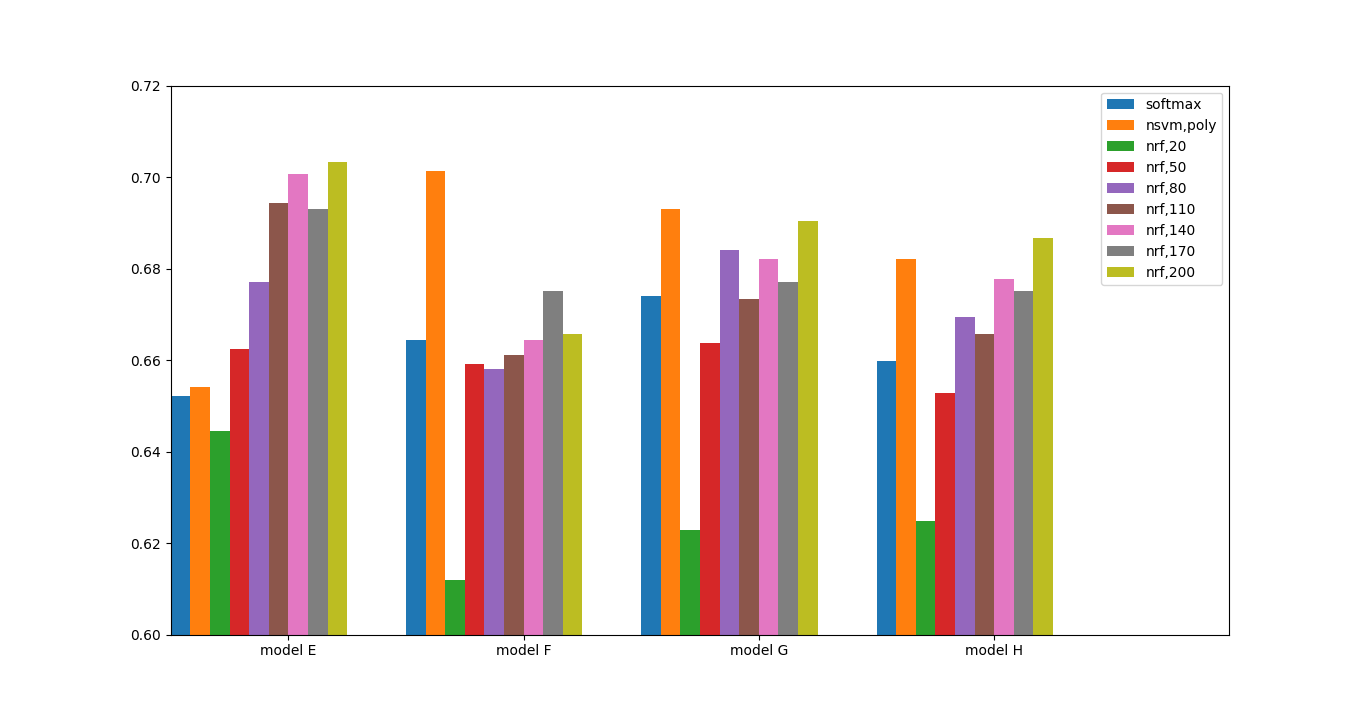
\includegraphics[scale=0.5]{../figures/CNN_rf1.png} \\
BP神经网络+CART。model A指$64\times64$,隐含层神经元个数为1000;model B指$96\times96$,隐含层神经元个数为1000;model C指$96\times96$,隐含层神经元个数为500;model D指$96\times96$,隐含层神经元个数为500,正则化系数为0.0001。
\end{center}
